\documentclass[a4paper, 12pt]{article}
\usepackage[utf8]{inputenc}
\usepackage{mathtools}
\usepackage{amssymb}
\usepackage{enumitem}
\usepackage{parskip}
\usepackage{xfrac}
\usepackage{xcolor}
\usepackage{booktabs}
\usepackage{graphicx}
\usepackage[export]{adjustbox}

\graphicspath{ {images/} }

\newcommand{\tr}{^{\mathsf{T}}}
\newcommand{\N}{\mathbb{N}}
\newcommand{\R}{\mathbb{R}}
\newcommand{\Z}{\mathbb{Z}}
\newcommand{\Q}{\mathbb{Q}}
\newcommand{\half}{\sfrac{1\!}2}
\DeclarePairedDelimiter\abs{\lvert}{\rvert}
\DeclarePairedDelimiter\floor{\lfloor}{\rfloor}
\DeclareMathOperator{\GL}{GL}
\DeclareMathOperator{\interior}{int}
\DeclareMathOperator{\closure}{cl}
\DeclareMathOperator{\aut}{Aut}
\DeclareMathOperator{\rank}{rank}

\setlist[enumerate, 1]{leftmargin=0pt, label=\textbf{\arabic*.}}

\begin{document}

\begin{enumerate}

\item \begin{enumerate}

\item \(Q_3\) has 4 eigenvalues listed below, where the entries of the eigenvectors are 1 if the corresponding piece of the cube is red and \(-1\) otherwise:
\begin{center}
\begin{minipage}{11cm}
\(\lambda_1=3\) spanned by \(\left\{\,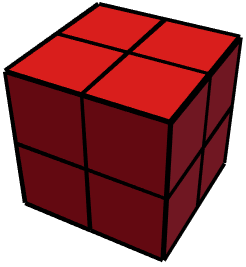
\includegraphics[valign=c, width=2cm]{1}\,\right\}\)

\(\lambda_2=1\) spanned by \(\left\{\,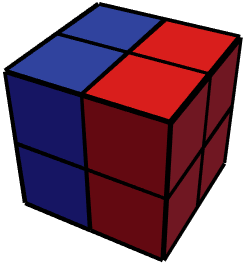
\includegraphics[valign=c, width=2cm]{2}, 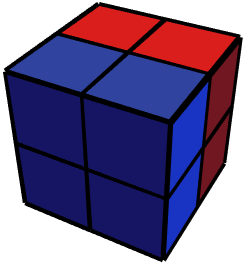
\includegraphics[valign=c, width=2cm]{3}, 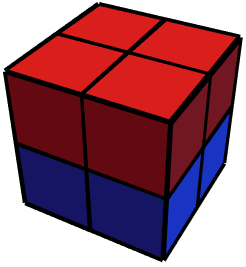
\includegraphics[valign=c, width=2cm]{4}\,\right\}\)

\(\lambda_3=-1\) spanned by \(\left\{\,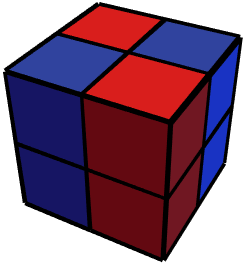
\includegraphics[valign=c, width=2cm]{5}, 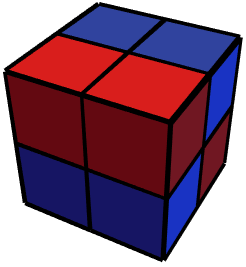
\includegraphics[valign=c, width=2cm]{6}, 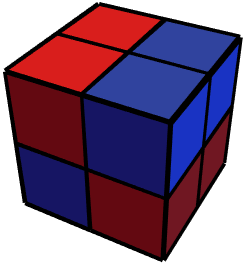
\includegraphics[valign=c, width=2cm]{7}\,\right\}\)

\(\lambda_4=-3\) spanned by \(\left\{\,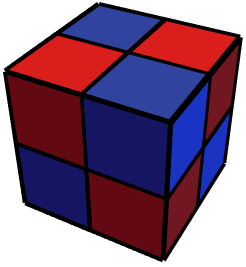
\includegraphics[valign=c, width=2cm]{8}\,\right\}\)
\end{minipage}
\end{center}

\item The Peterson graph is strongly regular with \(k=3\), \(\lambda=0\) and \(\mu=1\). By the proof of the rationality condition, 3 is an eigenvalue spanned by the all-ones vector, and the other two eigenvalues are 1 with multiplicity 5 and \(-2\) with multiplicity 4, with eigenspaces orthogonal to the all-ones vector.

The five rotations of
\begin{center}
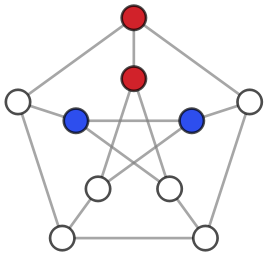
\includegraphics[valign=c, width=3cm]{pet1} \hspace{2em}\(\begin{array}{lcr}\text{red}&\to&1\\\text{blue}&\to&-1\\\text{white}&\to&0\end{array}\)
\end{center}
are linearly independent and so span the eigenspace of the eigenvalue 1

The five rotations of
\begin{center}
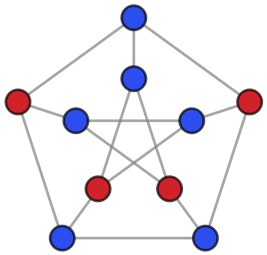
\includegraphics[valign=c, width=3cm]{pet2} \hspace{2em}\(\begin{array}{lcr}\text{red}&\to&3\\\text{blue}&\to&-2\end{array}\)
\end{center}
span a four-dimensional space since
\[\rank\begin{pmatrix}
-2&3&-2&-2&3&-2&-2&3&3&-2\\
3&-2&3&-2&-2&-2&-2&-2&3&3\\
-2&3&-2&3&-2&3&-2&-2&-2&3\\
-2&-2&3&-2&3&3&3&-2&-2&-2\\
3&-2&-2&3&-2&-2&3&3&-2&-2\\
\end{pmatrix}=4\]
and hence span the eigenspace of the eigenvalue \(-2\).

\item \(K_n\) is \((n-1)\)-regular so it has an eigenvalue \(n-1\) spanned by the all-ones vector. Also, \(K_n+I=J\) so \(K_n\) has an eigenvalue \(-1\) with \((n-1)\)-dimensional eigenspace the vectors whose entries sum to 0.

\item Let \(\omega\) be an \(n\)th root of unity. Then \(v\coloneqq(1,\omega,\omega^2\dots,\omega^{n-1})\) is an eigenvector of \(C_n\) with eigenvalue \(\omega+\omega^{-1}\) since the sum of the entries of the neighbours of a vertex with entry \(\omega^i\) is \(\omega^{i+1}+\omega^{i-1}=(\omega+\omega^{-1})\omega^i\). Note \(\omega^{-1}=\overline\omega\) so the eigenvalue \(\omega+\omega^{-1}\) is real.

If \(\omega\notin\{1,-1\}\) then the eigenvectors \(v\) and \(u\coloneqq(1,\omega^{n-1},\omega^{n-2},\dots,\omega)\) are linearly independent, so \(\omega+\omega^{-1}\) has multiplicity 2.

If \(\omega\) is 1 or \(-1\) the two corresponding eigenvectors coincide, so the eigenvector 2 is spanned by \((1,1,\dots,1)\) and the (possible) eigenvector \(-2\) is spanned by \((1,-1,1,-1,\dots,1,-1)\).

\end{enumerate}

\item The theoretical and actual independence numbers for the four graphs above are:
\begin{center}
\begin{tabular}{@{}ccc@{}}\toprule
Graph&Theorem 2.12 bound&Actual\\\midrule
\(Q_4\)&4&4\\
Peterson&4&4\\
\(K_n\)&1&1\\
\(C_n\)&\(\displaystyle \frac{n\cos\left(\frac{\floor*{\frac n2}}n2\pi i\right)}{\cos\left(\frac{\floor*{\frac n2}}n2\pi i\right)-1}\)&\(\displaystyle\floor*{\frac n2}\)\\
\bottomrule
\end{tabular}
\end{center}
When \(n\) is even the bound is met.

\item Let \(G\) be a graph such that every two distinct vertices have exactly two common neighbours.

\begin{enumerate}

\item Let \(u\) and \(v\) be distinct adjacent vertices of \(G\). For each neighbour \(u'\) of \(u\) there are exactly two common neighbours of \(u'\) and \(v\) --- one is \(u\) and the other we label as \(v'\). This induces a mapping \(\phi\colon u'\mapsto v'\) between the neighbourhoods of \(u\) and \(v\), excluding \(\{u,v\}\). Suppose \(\phi(a)=\phi(b)=c\). Then \(a\), \(b\) and \(v\) are three common neighbours of \(u\) and \(c\), so \(a=b\). Hence \(\phi\) is injective. By symmetry \(u\) and \(v\) have the same degree. Since \(G\) is connected and any two adjacent vertices have the same degree, \(G\) is regular.

The SRG parameters \(\lambda\) and \(\mu\) are 2, and by Lemma 2.13 we have
\begin{align*}
&k(k-\lambda-1)=(n-k-1)\mu\\
\implies\quad&n=\frac{k(k-3)}2+1+k.
\end{align*}
Hence \(G\) is strongly regular with parameters
\[(n,k,\lambda,\mu)=\bigg(\,\frac{k(k-3)}2+1+k,\,k,\,2,\,2\,\bigg).\]

\item By the rationality condition the two numbers
\begin{align*}
f,g&=\frac12\bigg(n-1\pm\frac{2k+(n-1)(\lambda-\mu)}{\sqrt{(\lambda-\mu)^2+4(k-\mu)}}\bigg)\\
&=\frac12\bigg(n-1\pm\frac{2k}{\sqrt{k-2}}\bigg)
\end{align*}
are integral. Hence \(\frac{2k}{\sqrt{k-2}}\) must be integral. It follows that \(k-2\) must be a square \(a^2\) so
\[\frac{2k}{\sqrt{k-2}}=\frac{2(a^2+2)}{a}=2a+\frac4a\]
which is integral only if \(a\) is 1, 2 or 4, which implies \(k\) is 3, 6 or 18. \(k=18\) does not satisfy the rationality condition so \(k\) is 3 or 6.

\item The \(k=3\) case is exhibited by \(K_4\). The \(k=6\) case is exhibited by \(K_4\square K_4\), since if if two vertices \(u,v\) are on the same row or column their common neighbours are the other two vertices on that row or column, and otherwise their common neighbours are the two vertices that complete the corners of a rectangle with \(u\) and \(v\).

\end{enumerate}

\item Let \(G\) be a connected graph of order \(n\) such that every vertex has degree at most 3.

\begin{enumerate}

\item Pick a vertex \(u\) in \(G\). Its orbit has size \(n\). Pick a neighbour \(v\) of \(u\). Under the stabiliser of \(u\) it must be mapped to a neighbour of \(u\) so its orbit has size at most 3.

Now pick a new point \(a\) adjacent to some previously chosen point \(b\). The point \(b\) is adjacent to some point chosen before it, so \(a\) must be sent to one of the other neighbours of \(b\). If \(b\) has degree \(2\) then \(a\) is fixed as the unique other neighbour of \(b\) and does not contribute to the size of the automorphism group, so pick a new \(a\) in the same way as before and repeat until you get a \(b\) with degree \(3\) (or the graph is exhausted). Then \(a\) must be sent to one of the two other neighbours of \(b\). This fixes the third neighbour of \(b\) as well. Since \(G\) is connected if we continue in this fashion we will eventually have fixed every point in \(G\). Each step of the process fixes at least two points and contributes a factor of at most 2 to the size of \(\aut G\). Hence the total contribution after every vertex has been fixed is at most \(2^{\frac{n-2}2}\). The size of \(\aut G\) is therefore at most \(3n2^{\frac{n-2}2}\)

\item \(K_4\) and \(K_{3,3}\) meet the bound since
\begin{gather*}
\abs{\aut K_4}=4!=3(4)2^{\frac{4-2}2}\\
\abs{\aut K_{3,3}}=2!\cdot3!\cdot3!=3(6)2^{\frac{6-2}2}.
\end{gather*}

\item If \(G\) has a vertex of degree less than 3, we can pick it as the first vertex in the process above and the bound becomes \(2n2^{\frac{n-2}2}\), so \(G\) must be 3-regular.

Similarly if \(G\) is not vertex-transitive we have \(m<n\) choices for the first vertex in the process above and the bound becomes \(3m2^{\frac{n-2}2}\), so \(G\) must be vertex-transitive.



\end{enumerate}

\end{enumerate}

\end{document}